
\documentclass[12pt]{article} 
\usepackage[utf8]{inputenc}
\usepackage[slovak]{babel}
\usepackage[hidelinks,unicode = true]{hyperref}
\usepackage{outline}
\usepackage{graphicx}
%\usepackage{biblatex}
%\addbibresource{literatura.bib}
\usepackage{cite}
\usepackage{caption}
%\usepackage{float} %upevneni tabulky
%\restylefloat{table}
\setcounter{secnumdepth}{3}
\setcounter{tocdepth}{3}
\usepackage{hyperref}
\hypersetup{
    colorlinks=true,
    linkcolor=blue,
    filecolor=magenta,      
    urlcolor=cyan,
}

%===========================================================================
\begin{document}           % Konec preambule a zároveň začátek vlastního textu
\begin{titlepage}
\centering
\Large \textbf{České vysoké učení technické v Praze }\\ Fakulta stavební
\vspace{2cm}

\begin{figure}[h!] %logoCVUT
\centering

\includegraphics[width=7cm]{./img/cvut.png}
\end{figure}
 
\Large \textbf{155UZPR Úvod do zpracování prostorových dat}
\vspace{1cm}

\LARGE  \textbf{ Nasazení vektorových dlaždic při tvorbě katastrální mapy}
\vspace{3cm}

\Large Bc. Linda Kladivová, Bc. Jana Špererová, Bc. Lukáš Kettner, Bc. Martin Hulín \\ 20.12.2019

 \thispagestyle{empty} %neočísluje první stránku
\end{titlepage}

\tableofcontents    % vytváří  Obsah 
\newpage %začne na nové stránce
%------------------------------------------------------------------------
\section{Úvod}



%------------------------------------------------------------------------
\clearpage 
\section{Popis a rozbor problému}

\subsection{Vektorvý a rastrový formát}
Každý z formátov publikácie priestorových dát má svoje výhody a nevýhody. Je potreba dobre zvážiť umýsel, možnosti a výsledný cieľ publikácie. Rastrové dlaždice majú v porovnaní s vektorovými jednoduchšiu dátovú štruktúru a spracovanie rastrových dát je vo väčšine prípadov jednoduchšie. Veľkou nevýhodou dát v rastrovom formáte sú obmedzené možnosti práce s datami, kedy pri porovnaní s vektorovými dátami pracujeme s obrazom javu a nie konkrétnymi geoprvkami. Ďalšou nevýhodou rastrových dlaždíc je ich veľkosť. Vzhľadom na využitie práce, riešenie má byť aplikované pre dáta celého územia Českej republiky, je práve veľkosť kľúčovým faktorom, ktorý hovorí v prospech vektorových dlaždíc. Z hladiska úložiska vektorové dlaždice zaberajú kapacitne niekoľkonásobne menší (väčšinou) priestor úložiska. Z tohto faktu plynie ďalšia výhoda pri použiti vektorových dlaždíc, úspora datového toku na klientovi, vykreslujú sa dlaždice, ktoré sú v aktuálnom pohľade mapy. 
\newline Ďalším podstatným plusom oproti rastrovým dlaždiciam je možnosť vektorového formátu niesť topologickú informáciu, ktorú môže užívateľ využiť pri následnej práci s dátami a vykonávaní rozličných analýz. Jedným z príkladov je možnosť vykonávať úpravy priamo na strane klienta,  bez nutnosti interakcie so serverom. Táto možnosť je užitočná pri projektoch v oblasti open source mapovania a práci s využitím mapovej služby priamo v teréne. 
\newline K výhodám vektorových dlaždíc patrí aj kartografická generalizácia. V závislosti na úrovni priblíženia (merítku) je možné nastaviť optimalizáciu zobrazenia vektorových dlaždíc. Jednotlivé geoprvky je možné zlúčiť, zjednodušiť či agregovať, tak aby podrobnosť geometrie a atribútového obsahu dlaždíc odpoveda úrovni priblíženia.
\newline Jednou z ďalších výhod vektorových dátach je možná individuálna štylizácia dát na strane klienta, presne podľa jeho požiadavkov, bez toho aby dáta na serveri museli byť zmené.
\newline V prípade modelového príkladu z praxe. Pokiaľ by sme chceli na mobilnom zariadení, v lokalite so slabším internetovým pripojením vykonať jednoduchú analýzu nad mapou vytvorenou z rastrových dlaždíc, sme takmer bez šance na úspech. V prípade použitia vektorových dlaždíc bude možné túto analýzu vykonať.

\subsection{Súčasný stav mapového serveru Marushka}

V súčasnom stave mapový server Marushka slúži k uloženiu, poskytovaniu a aktualizácii mapových dát na území Českej republiky. Všetky dáta publikované touto aplikáciou sú uložené v databázy Informačného systému katastru nemovitostí (ISKN) a v databázy Informačného systému územnej identifikácie (ISÚI). V rámci týchto dvoch databází prebiehajú všetky aktualizácie zobrazených prvkov. Na tieto databáze je následne napojená Publikačná databáza a v nej prebiehajú úpravy geometrií v pravidelných dvojhodinových cykloch. Úpravy sa týkajú zväčša transformácie geometrie , aby bolo možné jej optimálnejšie zobrazovanie a publikácia. Celá logika postupu je na základe databázovej úrovne a je realizovaná pomocou PL/SQL skriptov. Takto upravené dáta sú automaticky exportovaná do WKB súborov. Z týchto preddefinovaných súborov prebieha samotná publikácia dát vo forme rastrových dlaždíc. K aktualizácii katastrálnej mapy dôjde v celom katastrálnom území, pokial sa v ňom objaví zmena.

\begin{center}
   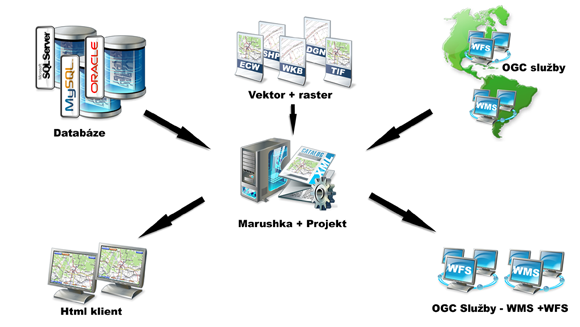
\includegraphics[width=12cm]{./img/Marushka1.png}
   \captionof{figure}{Mapový server Marushka}
\end{center}

 Pre lepšie porozumenie je potrebné objasniť, čo je to WKB súbor. Mapový server Marushka nativne pracuje s týmto vektorovým formátom, Well known Binary (WKB, štandard konsorcia OGC). Tento formát je používaný aj pre implementáciu databázového priestorového úložiska, ktoré je kompatibilné s produktami fy GEOVAP(Geostore), prípadne pre export akéhokoľvek skladu do tzv. file cash. 
 \newline Nad súbormi WKB je možné vybudovať viacúrovňový priestorový index reprezentovaný štruktúrou R-Tree. Tento index výrazne zefektívni priestorový prístup k jednotlivým geometrickým elemoentom. Podrobnejšie informácie je možné nájsť na oficiálne stránke  \href{http://geovap.q2.cz/marushka/cz/produkty-a-sluzby/categoryId/3/souborove-vektorove-formaty-/popis/architektura/2#item15}{ serveru Marushka}.
 \newline Využitie vektorových dlaždíc na mapovom serveri Marushka by viedlo k zjednodušeniu aktualizácie katastrálnej mapy. Aktualizovala by sa len základná dlaždica, v ktorej sa prvok nachádza. To by vylúčilo nutnosť aktualizovať celé katastrálne územie, tým by sa výrazne znížila časová náročnosť pre aktualizáciu dát a aktualne dáta na mapovom serveri Marushka by mali užívatelia k dispozícii takmer ihneď po úprave.



%------------------------------------------------------------------------
\clearpage
\section{Popis a formát vstupních dat}
Našimi počátečními vstupními daty jsou data katastrální mapy ve formátu shapefile. Pro automatické stažení dat po katastrálních územích je na stránkách \href{http://services.cuzk.cz/shp/ku/QGIS-plugin/QGIS_verze-3.x/}{Services ČÚZK} k dispozici zásuvný modul pro hromadné stahování dat KM ve formátu .shp. Zadáním příslušného textového souboru s připraveným seznamem katastrálních území dojde ke stažení dat a jejich rozčlenění po katastrálních území. Shapefily katastrální mapy jsou přibližným obrazem publikační databáze na ČÚZK. Vzhledem k tomu, že v publikační databázi může být v jedné tabulce i vícero sloupců s různými typy geometrií, neodpovídají názvy shapefilů názvům tabulkám v publikační databázi. Aby bylo zřejmé, o jaký konkrétní prostorový typ dat se jedná, jsou jednotlivé shapefily pojmenovány podle svých typů. Jednotlivé typy jsou uvedeny na příkladu vrstvy PARCELY\_KN: 

\begin{itemize}
\item PARCELY\_KN\_B.shp $\rightarrow$ body parcel (multipoint)
\item PARCELY\_KN\_DEF.shp $\rightarrow$ definiční body parcel (multipoint)
\item PARCELY\_KN\_L.shp $\rightarrow$ linie parcel (multilinestring)
\item PARCELY\_KN\_P.shp $\rightarrow$ polygon parcel (multipolygon)
\item PARCELY\_KN\_T.shp $\rightarrow$ text (multipoint)
\end{itemize}

Shapefile je datový formát pro ukládání vektorových prostorových dat, který se skládá s několika povinných a doplňkových souborů. Hlavní soubor .shp obsahuje seznam lomových bodů dané geometrie. Databázový soubor .dbf obsahuje popisné atributy jednotlivých geometrí, které v tomto případě kopírují popisné informace v tabulkách v publikační databázi. Tyto dva jmenované soubory jsou propojeny pomocí dalšího posledního povinného souboru .shx. U všech vrstev je obsažen ještě soubor .prj, který je ve všech případech stejný. Obsahuje definici souřadnicového systému a projekce (EPSG kód 5514). 

\clearpage 
%------------------------------------------------------------------------
\section{Výstupní data, formát a popis}


%------------------------------------------------------------------------
\clearpage 
\section{Pracovný postup}




%-------------------------------------------------------------------------
\clearpage
\section{Záver, možné a neriešené problémy}
Výsledkom práce je ...

\newpage
%-------------------------------------------------------------------------

%Zobrazeni seznamu obrazku
%\cleardoublepage
%\addcontentsline{toc}{chapter}{\listfigurename}
\listoffigures

%-------------------------------------------------------------------------

\listoftables

%-------------------------------------------------------------------------
\nocite{*}
%\printbibliography
\bibliography{literatura}{}
\bibliographystyle{plain}
%-------------------------------------------------------------------------
    
\end{document}             % Konec dokumentu.
